\fullsys (\sys) is the abstraction of a group of batteryless intermittent sensors. \sys seeks to offer continuous sensing despite its reliance on ambient energy: an unpredictable and marginal power source. 
%orchestrates its nodes power cycles using a distributed approach (instead of relying on a master powerful node to coordinate coalesced nodes activities). 
%\sys seeks maximum time span of its underlying coalesced nodes through a distributed approach instead of a master node that orchestrates coalesced nodes on/off cycles. 

\subsection{\fullsys Nodes}
As Figure~\ref{fig:cisPwrCycle} shows, an intermittent node can have two or three distinct energy consumption rates. If the node does a polling-based sensing then its energy consumption, generally, switches between zero when charging and a maximum when it activates its microcontroller  (we assume that the microcontroller is the dominate energy consumer module of the node). However, in event-based sensing a node puts its microcontroller into low power mode and wait (or listen) for an external event to make up the microcontroller. This idle listening mode adds a third energy consumption level which has an important impact on the design of the \sys.
%
\begin{figure}[t]
	\centering
		\begin{subfigure}{\columnwidth}
			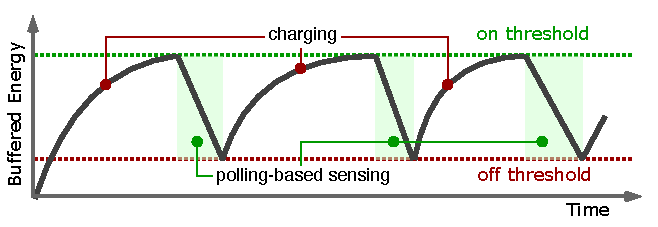
\includegraphics[width=\columnwidth]{figures/PowerCycleIntermittentSystem}
			\caption{When \sys does polling-based sensing, its energy consumption profile has, generally, two distinct levels.}
			\label{fig:solarPwrCoIS}
	\end{subfigure}
	\begin{subfigure}{\columnwidth}
		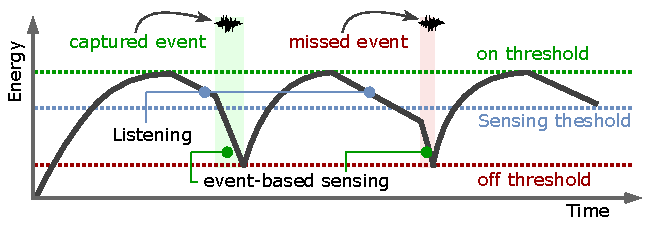
\includegraphics[width=\columnwidth]{figures/PowerCycleIntermittentSensor}
		\caption{When \sys does event-based sensing---staying in low power mode listening for an external event to happen---, its energy consumption profile has three distinct levels.}
		\label{fig:solarPwrCoIS}
\end{subfigure}
		\caption{\fullsys energy consumption profile for different sensing strategies}
		\label{fig:cisPwrCycle}
\end{figure} 
%
\subsection{\fullsys On-time}
To distribute intermittent nodes' uptimes, two broad controlling methods can be imagined:
\begin{enumerate}[wide, labelwidth=!, labelindent=0pt]
		\item An explicit uptimes control method which requires inter-nodes communication; uptimes chaining techniques, to enable message passing across different time slots; and number of active nodes estimation per a time slot. Once a node estimates the number of active nodes, within its uptime, it must decide, based on per defined criteria, on leaving this power cycle or maintaining it. A node can change its on/off cycle relative to other nodes' cycles by either increasing (or decreasing) its power consumption to shorten (or lengthen) its uptime and shift its power cycle. 
		\item An implicit uptimes control method seeks to use a random process to "ideally" uniformly distribute nodes' on/off cycles over the \sys's power cycle: when all the nodes complete their individual power cycles.  
\end{enumerate}
There is a clear trade-off between the aforementioned methods. While the explicit control method provide a fine control over the system distribution, the implicit method does not suffer from control messages exchange overhead. Although the implicit method is relatively simple to implement and explore, the explicit control method is not a far fetched idea (the recent advancements in passive light~\cite{marco} and ambient radio waves backscattering~\cite{} that enable extremely energy efficient passive communication for batteryless devices). However, we opt to explore the implicit distribution control methods as we think that the uptimes chaining technique and number of nodes per a time slot estimation, required by the explicit control method, are not trivial tasks and deserve there own study. Additionally, the hardware used to demonstrate the feasibility of passive light communication and ambient RF backscattering are not open source and re-making it is beyond the scope of this study.

%Effective message passing between batteryless nodes requires an ultra low power communication regime. Thanks to the recent advancements in passive visible light communication~\cite{Marco} and ambient radio frequency backscattering~\cite{} that demonstrate the feasibility of extremely energy efficient communication between batteryless nodes. Once messages exchange is possible, an intermittent node's duty is to estimate the number of active nodes in its time slot and to decide on leaving this power cycle of maintaining it (Figure~\ref{xxx}). Nodes can influence their power cycles by altering their loads---a node can shorten its uptime (and consequently its power cycle) by increasing its energy consumption. Inversely, a node's low power consumption mode extends its uptime and lengthen its on/off cycle. 
\paragraph{Light-based Implicit Nodes' Uptimes Control}
%
%
As Figure~\ref{fig:solarPwrCoIS} shows light powers tiny sensory nodes intermittently. It also indicates that \sys availability increases as more intermittent nodes added. The dashed line is the simulated time coverage of the system as the intermittent nodes power-ups are uniformly distributed. By comparing the measured \sys's availability line graphs to the simulated one we can conclude that harvesting solar power of artificial light provides sufficient randomness to distribute the coalesced nodes uptimes uniformly. Figure~\ref{fig:sysDutyCycle} shades more light on this observation. It show that each node has it own unique duty cycle. The little differences between the duty cycles causes them to have a "near" constant shifts relative to each other which in turn causes the system to nodes' uptimes to have near uniform distribution.

\subsection{\fullsys Power States}
From~\ref{fig:solarPwrCoIS} we can identify four operational stages for a \sys:
\begin{enumerate}
		\item \textit{Under-targeted energy conditions}---a \sys should be designed for near worst case energy conditions in order to comply with design requirements. However, a solar powered \sys, for example,  will come to a perpetual power down in the darkness. In general, for under-targeted energy conditions the system behavior is undefined.
		\item \textit{targeted energy conditions}---in these energy conditions the \sys should work intermittently and have sufficient randomness to distribute its intermittent nodes' power cycles to meet the desired availability percentage. 
\end{enumerate}


To meet a certain system availability, the system needs to be design for low energy conditions (i.e. artificial light).Depending on the ambient energy conditions, a \sys's power can vary significantly.  Generally, we can define four operational conditions that a \sys can experience.

\begin{figure}
		\centering
		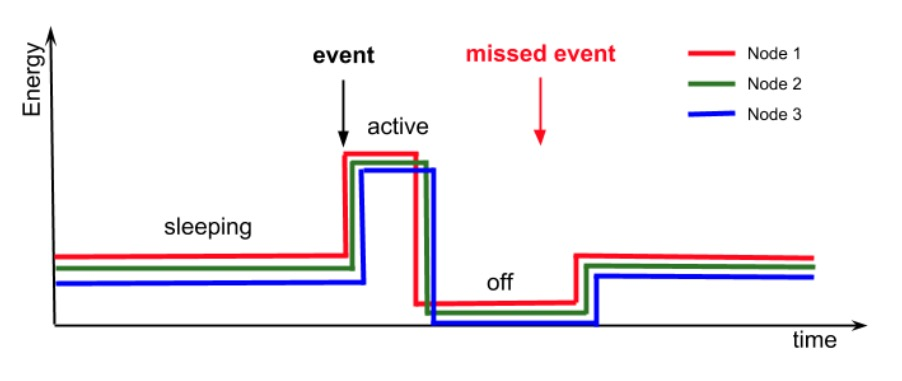
\includegraphics[width=\columnwidth]{figures/noRandomization}
		\caption{\todo{Placeholder} No randomization}
		\label{fig:noRand}
\end{figure} 

\begin{figure}
		\centering
		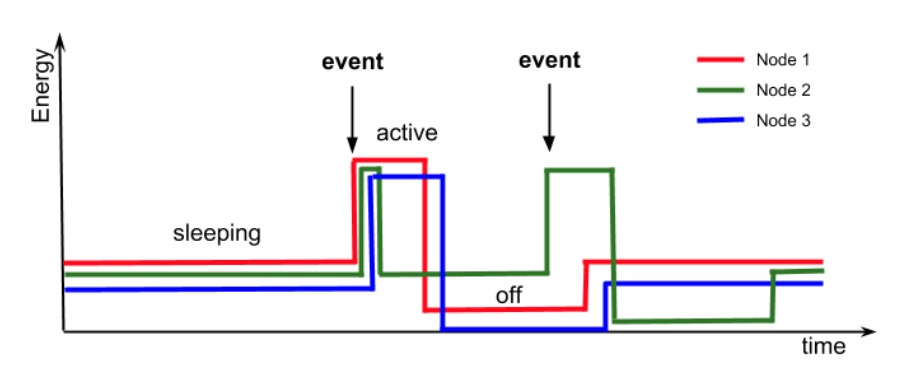
\includegraphics[width=\columnwidth]{figures/randomization}
		\caption{\todo{Placeholder} Randomization}
		\label{fig:noRand}
\end{figure} 

\begin{figure}
		\centering
		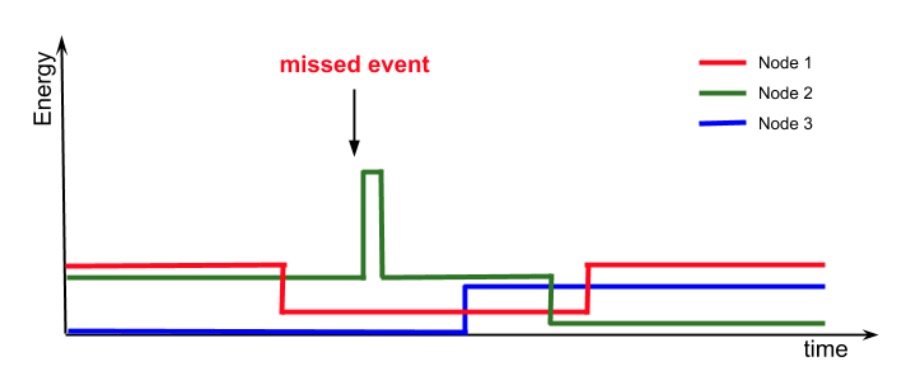
\includegraphics[width=\columnwidth]{figures/randomizationSideEffect}
		\caption{\todo{Placeholder} Randomization side effect}
		\label{fig:noRand}
\end{figure} 


